%%%%%%%%%%%%%%%%%%%%%%%%%%%%%%%%%%%%%%%%%%

\chapter{Monte Carlo simulations of UCN transport and spin transport}\label{chap:simulations}

%%%%%%%%%%%%%%%%%%%%%%%%%%%%%%%%%%%%%%%%%%

Monte Carlo methods are a broad class of algorithms based on the repeated sampling of appropriate random distributions. They can be used for a wide variety of applications, from calculating $\pi$ to modelling ferromagnetism with the Ising model. For the LANL nEDM the primary application of Monte Carlo algorithms is for simulating UCN transport and UCN spin transport in the experiment, where UCN are sampled from an initial velocity and spatial distribution and allowed to propagate freely. Monte Carlo methods lend themselves well to parallelization, so long as the distribution sampling is sufficiently randomized (i.e. not correlated or periodic). Adding computing power, namely more threads, to a Monte Carlo simulation reduces runtime and adds statistical accuracy. For this reason, many of the simulations presented in this chapter were run with the supercomputing clusters at \acrshort{iu}. Ultimately, a Monte Carlo simulation is only as accurate as the physics entered into the model, and requires both careful benchmarking and validation with experimental data in order to obtain a physically meaningful result.

Section~\ref{sec:pentrack} describes \pentrack, a powerful simulation tool for UCN experiments. In Sec. \ref{sec:switcher_wye_transport_monte_carlo}, we use it to model the UCN transport measurements on the West beamline (Chap.~\ref{chap:fall2021}) to better understand the discrepancy in counted UCN by beam height detectors on the switchers. Section~\ref{sec:switcher_wye_transport_monte_carlo} demonstrates UCN transport from the UCN source to the LANL nEDM apparatus on the North beamline. We examine the effects of depolarization and diffusivity in the switcher wye on spin asymmetry of stored UCN. Section~\ref{sec:1D_random_walk} introduces an alternative to comprehensive UCN transport simulations --- a 1D random walk model for UCN transport into a precession cell, which has the benefit a smaller parameter space.

%%%%%%%%%%%%%%%%%%%%%%%%%%%%%%%%%%%%%%%%%%

\section{PENTrack}\label{sec:pentrack}

%%%%%%%%%%%%%%%%%%%%%%%%%%%%%%%%%%%%%%%%%%

\pentrack \cite{schreyer_pentrack} is a simulation tool written in C++ for UCN experiments developed by Wolfgang Schreyer. It supports many excellent features, including:
%
\begin{itemize}
    \item Arbitrary experimental geometries defined by STL files
    \item Simulation of neutron trajectories under the influence of gravity, magnetic field gradients, etc.
    \item Diffuse surface reflection and transmission with Lambertian and micro roughness models (Sec.~\ref{sec:diffuse_reflections})
    \item Arbitrary analytical and numerical electromagnetic fields, with time dependence
    \item Definition of multiple material types via real and imaginary optical potentials~(Sec.~\ref{sec:ucn_matter_int})
    \item Relativistic spin tracking with the BMT equation (Sec.~\ref{sec:BMT_equations}). Spin tracking of high speed particles such as electrons, protons, etc. are supported.
    \item Simulation of neutron decay and the tracking of resulting protons and electrons
    \item Simulation of xenon, \hg, and additional user-defined particles
    \item Output to ROOT or HDF binary formats
\end{itemize}
%
The numerical integration method utilized by \pentrack is a 5th-order Dortmund Prince algorithm~\cite{numerical_recipes}. The pseudo-random generator is the 64-bit Mersenne Twister 19937 algorithm. The seed is generated with a nanosecond resolution time stamp or can be provided directly, which makes \pentrack suitable for running in a multi-threaded mode.

Perhaps most importantly, the \pentrack code base is clearly written and readable, making contributing to it widely accessible. The simulation code is available at [\url{https://github.com/wschreyer/PENTrack}].

%%%%%%%%%%%%%%%%%%%%%%%%%%%%%%%%%%%%%%%%%%

\section{Simulation of UCN rate change from switcher height differential}\label{sec:switcher_height_monte_carlo}

%%%%%%%%%%%%%%%%%%%%%%%%%%%%%%%%%%%%%%%%%%

 \begin{figure}
    \centering
    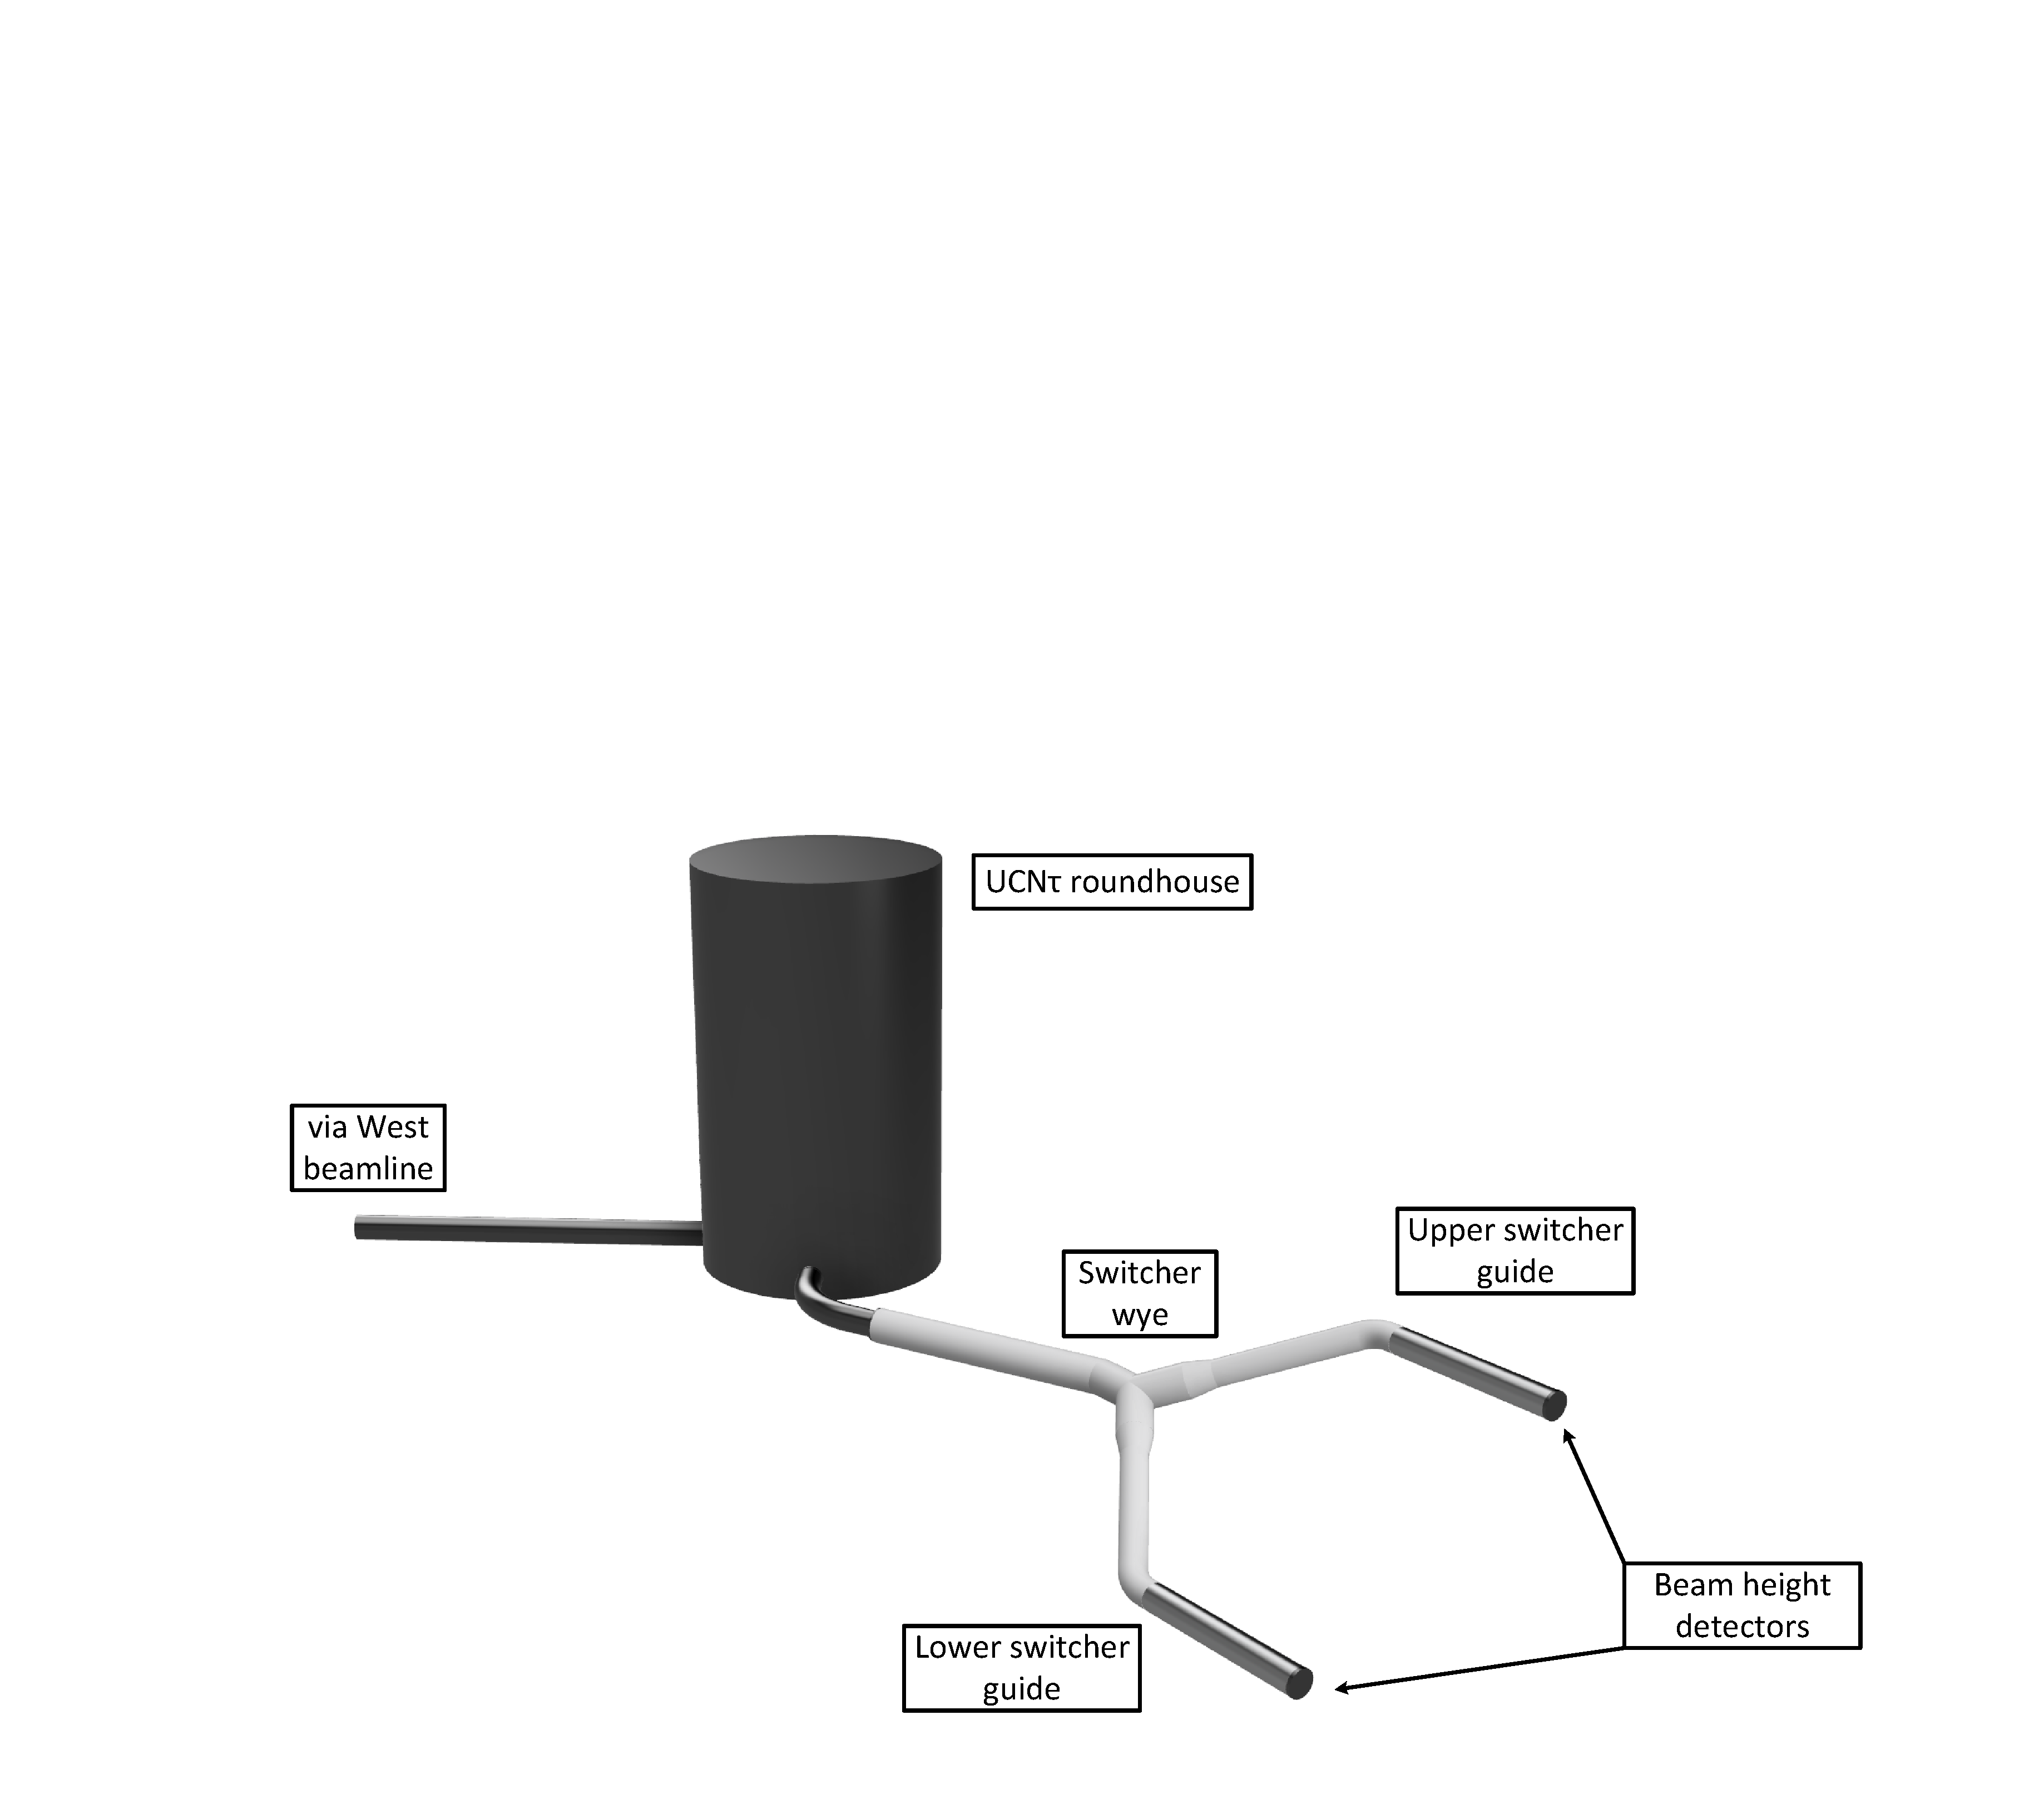
\includegraphics[width=0.8\textwidth]{figures/2021_west_beamline_pentrack.pdf}
    \caption
     {Experimental geometry of the switcher wye and UCN$\tau$ roundhouse (Chap.~\ref{chap:fall2021}) used in a \pentrack simulation to examine UCN transmission through the switcher wye.}
    \label{fig:west_beamline_pentrack_geometry}
\end{figure}

\begin{figure}
\centering
%subfigure width gets "multiplied" by includegraphics width
\begin{subfigure}{.5\textwidth} 
  \centering
  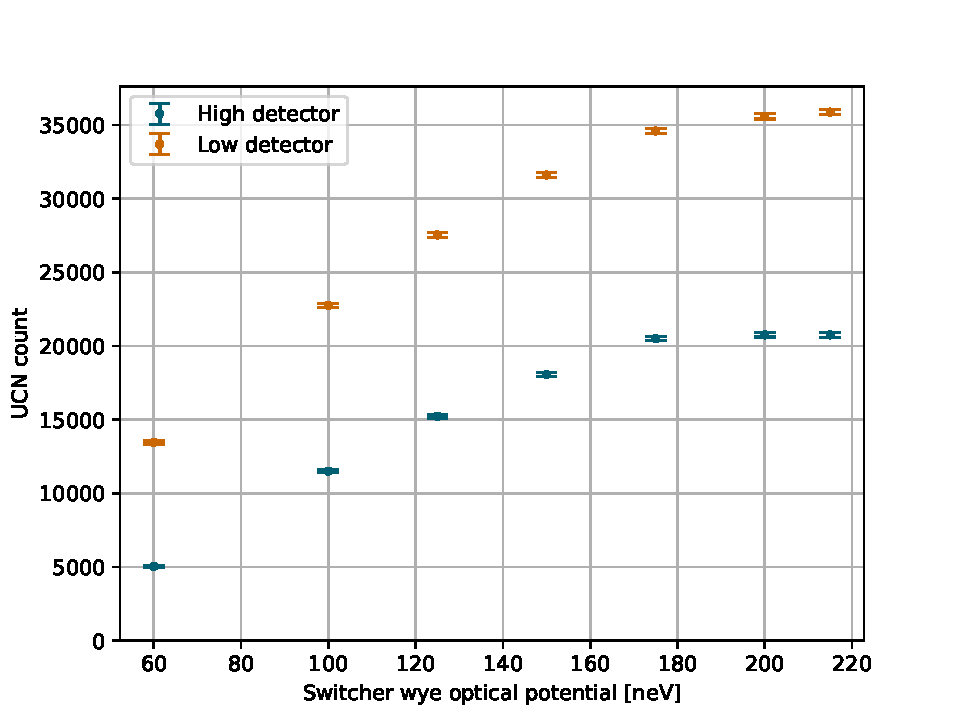
\includegraphics[width=\textwidth]{figures/fermi_sweep_y_counts.pdf}
  \caption{}\label{subfig:y_fermi_sweep_counts}
\end{subfigure}%DO NOT REMOVE THIS '%'
\begin{subfigure}{.5\textwidth}
  \centering
  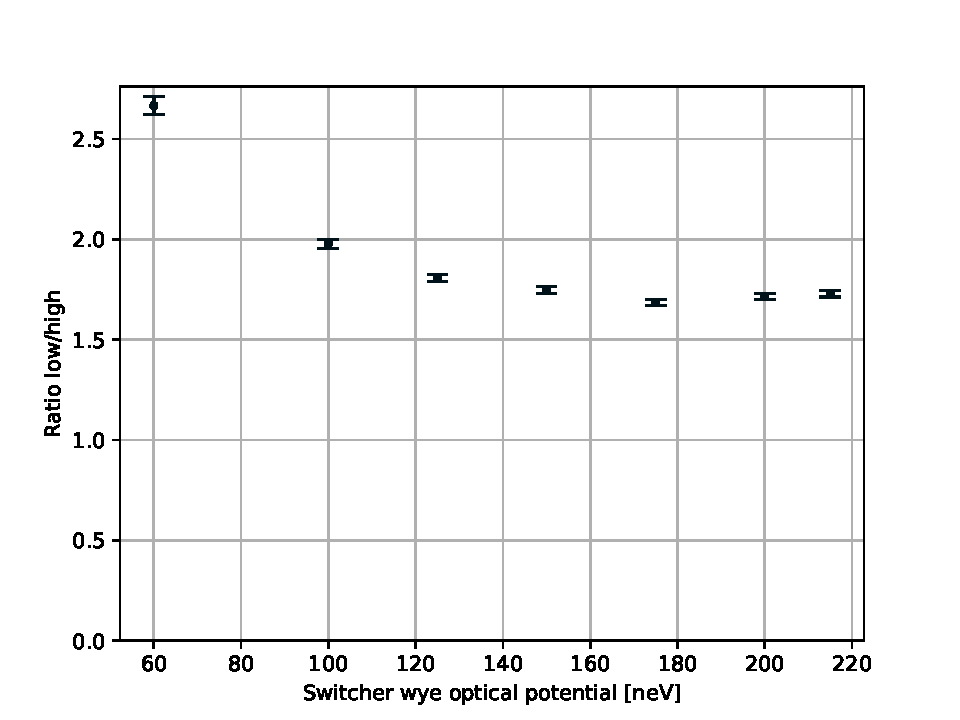
\includegraphics[width=\textwidth]{figures/fermi_sweep_y_ratio.pdf}
  \caption{}\label{subfig:y_fermi_sweep_ratio}
\end{subfigure}
\caption
{\textbf{(\subref{subfig:y_fermi_sweep_counts})} Results of the flow through simulation through the West beamline configuration for various switcher wye optical potentials Sec.~\ref{sec:switcher_height_monte_carlo}. Counted UCN in beam height detectors mounted at the heights of upper and lower switchers. \textbf{(\subref{subfig:y_fermi_sweep_ratio})} Ratio in counts of the lower switcher beam height detector to the upper switcher beam height detector}
\label{fig:y_fermi_sweep_ratio_pentrack}
\end{figure}


\begin{figure}
\centering
%subfigure width gets "multiplied" by includegraphics width
\begin{subfigure}{.5\textwidth}
  \centering
  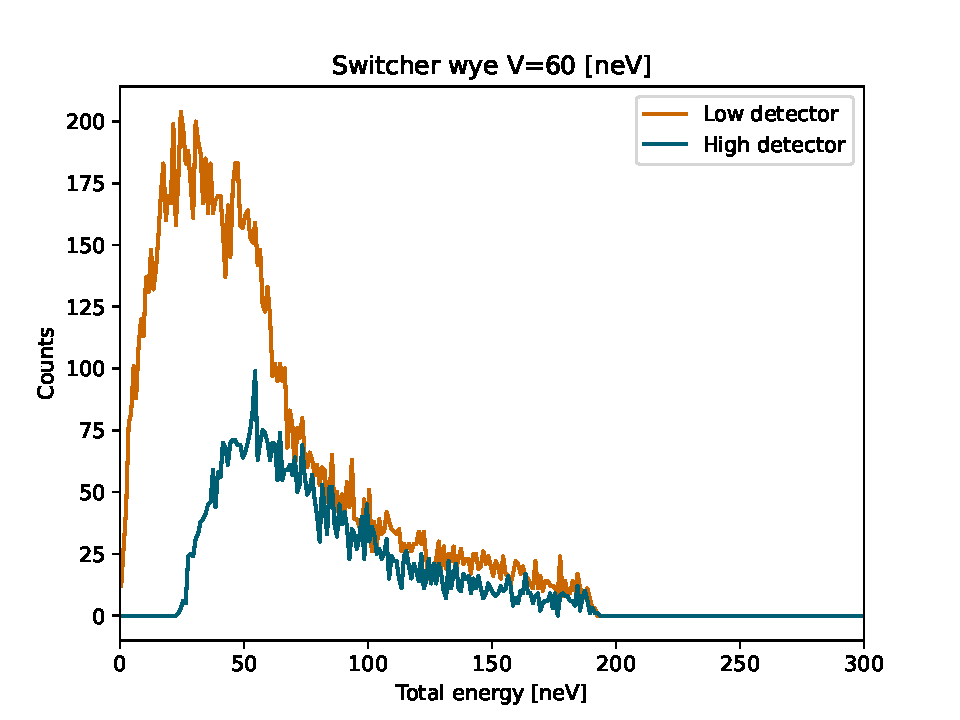
\includegraphics[width=\textwidth]{figures/fermi60_E_hist.pdf}
  \caption{}\label{subfig:V=60_simul}
\end{subfigure}%DO NOT REMOVE THIS '%'
\begin{subfigure}{.5\textwidth}
  \centering
  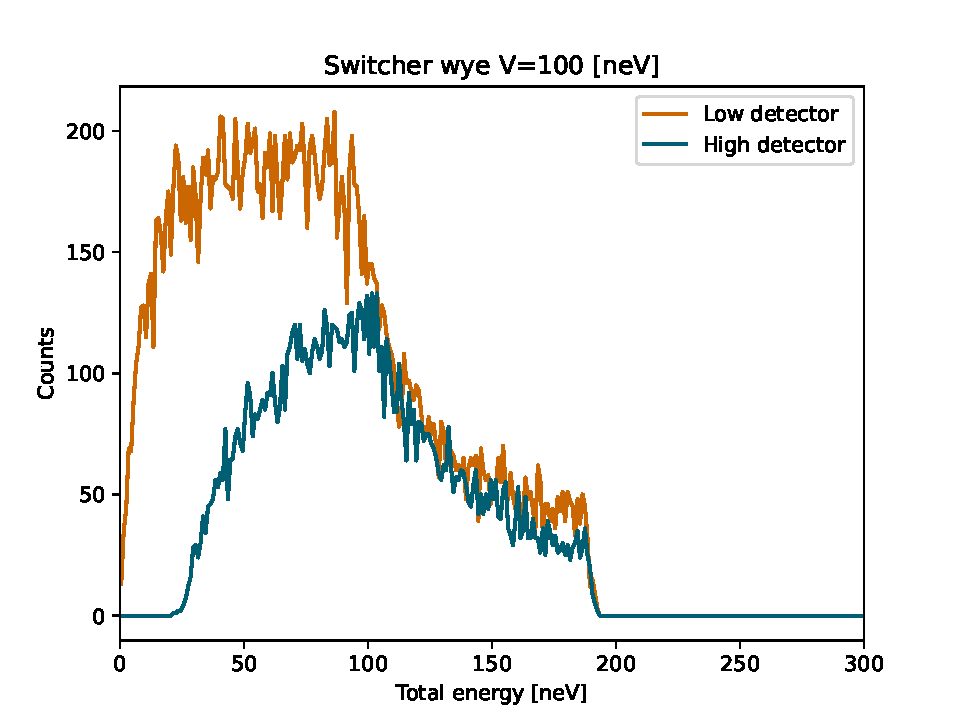
\includegraphics[width=\textwidth]{figures/fermi100_E_hist.pdf}
  \caption{}\label{subfig:V=100_simul}
\end{subfigure}
\begin{subfigure}{.5\textwidth}
  \centering
  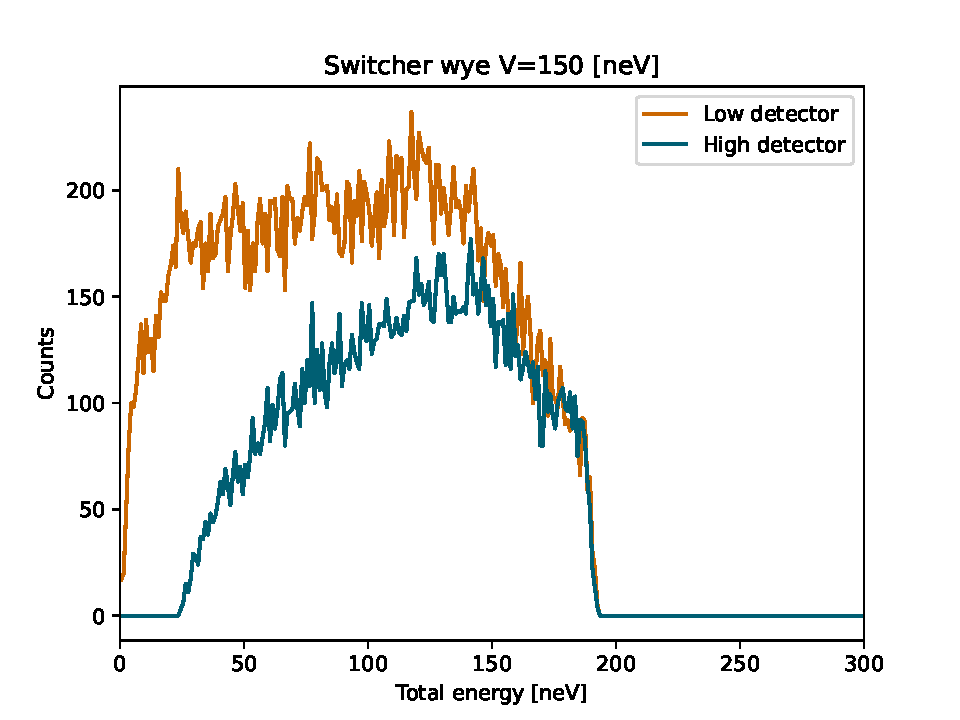
\includegraphics[width=\textwidth]{figures/fermi150_E_hist.pdf}
  \caption{}\label{subfig:V=150_simul}
\end{subfigure}%DO NOT REMOVE THIS '%'
\begin{subfigure}{.5\textwidth}
  \centering
  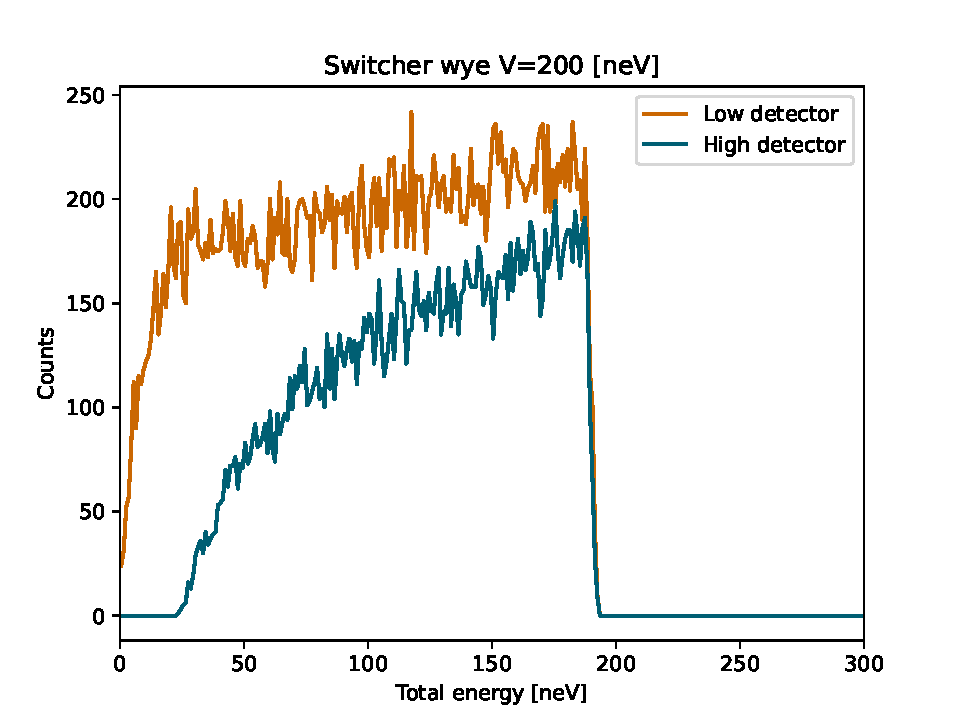
\includegraphics[width=\textwidth]{figures/fermi200_E_hist.pdf}
  \caption{}\label{subfig:V=200_simul}
\end{subfigure}
\caption
{UCN total energy spectra from the flow through simulation of the West beamline geometry for various switcher wye optical potentials. See discussion in Sec.~\ref{sec:switcher_height_monte_carlo}.}
\label{fig:y_E_hist_pentrack}
\end{figure}

We first use \pentrack to simulate the transport of UCN on the West beamline to examine the discrepancy of UCN count rate on beam height detectors (Sec.~\ref{sec:2021_ucn_transport_switchers}). As summarized by Tab.~\ref{tb:2021_transport}, the beam height detector on the lower switcher has a factor of $\approx1.5$ higher UCN count rate than the beam height detector on the upper switcher.

The geometry simulated is shown in Fig.~\ref{fig:west_beamline_pentrack_geometry}. UCN with a $v^2\,dv\,(=E^{1/2}\,dE)$ (Sec.~\ref{subsec:storageCurves}) input distribution and an isotropic angular distribution began on the West beamline. The initial UCN energy was set in the range of 0--\qty{188}{\nano\eV} due to the SS components in the roundhouse (Sec.~\ref{sec:single_arm_flow_through_west_2021}). The material of the geometry was generally set to NiP (Tab.~\ref{tb:optical_potentials}), and the probability of Lambertian diffuse bounces was set to 0.05, consistent with the value reported in Ref.~\cite{saunders_performance_2013}. Two perfect UCN beam height detectors were placed at the end of the switcher guides. The real optical potential $V_\text{wye}$ of the switcher wye component was varied (imaginary component $W_\text{wye}=0$).

Figure~\ref{subfig:y_fermi_sweep_counts} show the UCN counted by the beam height detectors as a function of $V_\text{wye}$. Expectedly, low wye optical potentials transmitted fewer total UCNs to the beam height detectors because UCN could not be contained unless the angle of incidence was glancing. Optical potentials higher than the maximum \qty{188}{neV} of the input spectrum did not exhibit a large difference in UCN counted. Interestingly, from Fig.~\ref{subfig:y_fermi_sweep_ratio}, we immediately see that the ratio in counted UCN for $V_\text{wye}\geq \qty{150}{neV}$ is already $\approx 1.75$ without the need to tune parameters such as input distribution (i.e. $v^3\,dv\,(=E\,dE)$), maximum input energy of UCN, or guide diffusivity.

Figure~\ref{fig:y_E_hist_pentrack} plots the total energy of UCN in each beam height detector for selected $V_\text{wye}$. In all cases we observe the expected \qty{25}{n\eV} gravitational potential step that limited lower energy UCN from reaching the upper detector (switcher wye dimensions in Fig.~\ref{fig:switcher_stand_measurements}). For each value of $V_\text{wye}$, we see a distinct cutoff corresponding to the optical potential, after which counts of UCN with higher energies drop off rapidly.

While free parameters in the simulation can be further tuned, this demonstration was enough to assuage fears of exposed Al or otherwise compromised coating on the switcher wye. 

%%%%%%%%%%%%%%%%%%%%%%%%%%%%%%%%%%%%%%%%%%

\section{Simulation of transport from the UCN source into the apparatus}\label{sec:switcher_wye_transport_monte_carlo}

%%%%%%%%%%%%%%%%%%%%%%%%%%%%%%%%%%%%%%%%%%

\begin{figure}
    \centering
    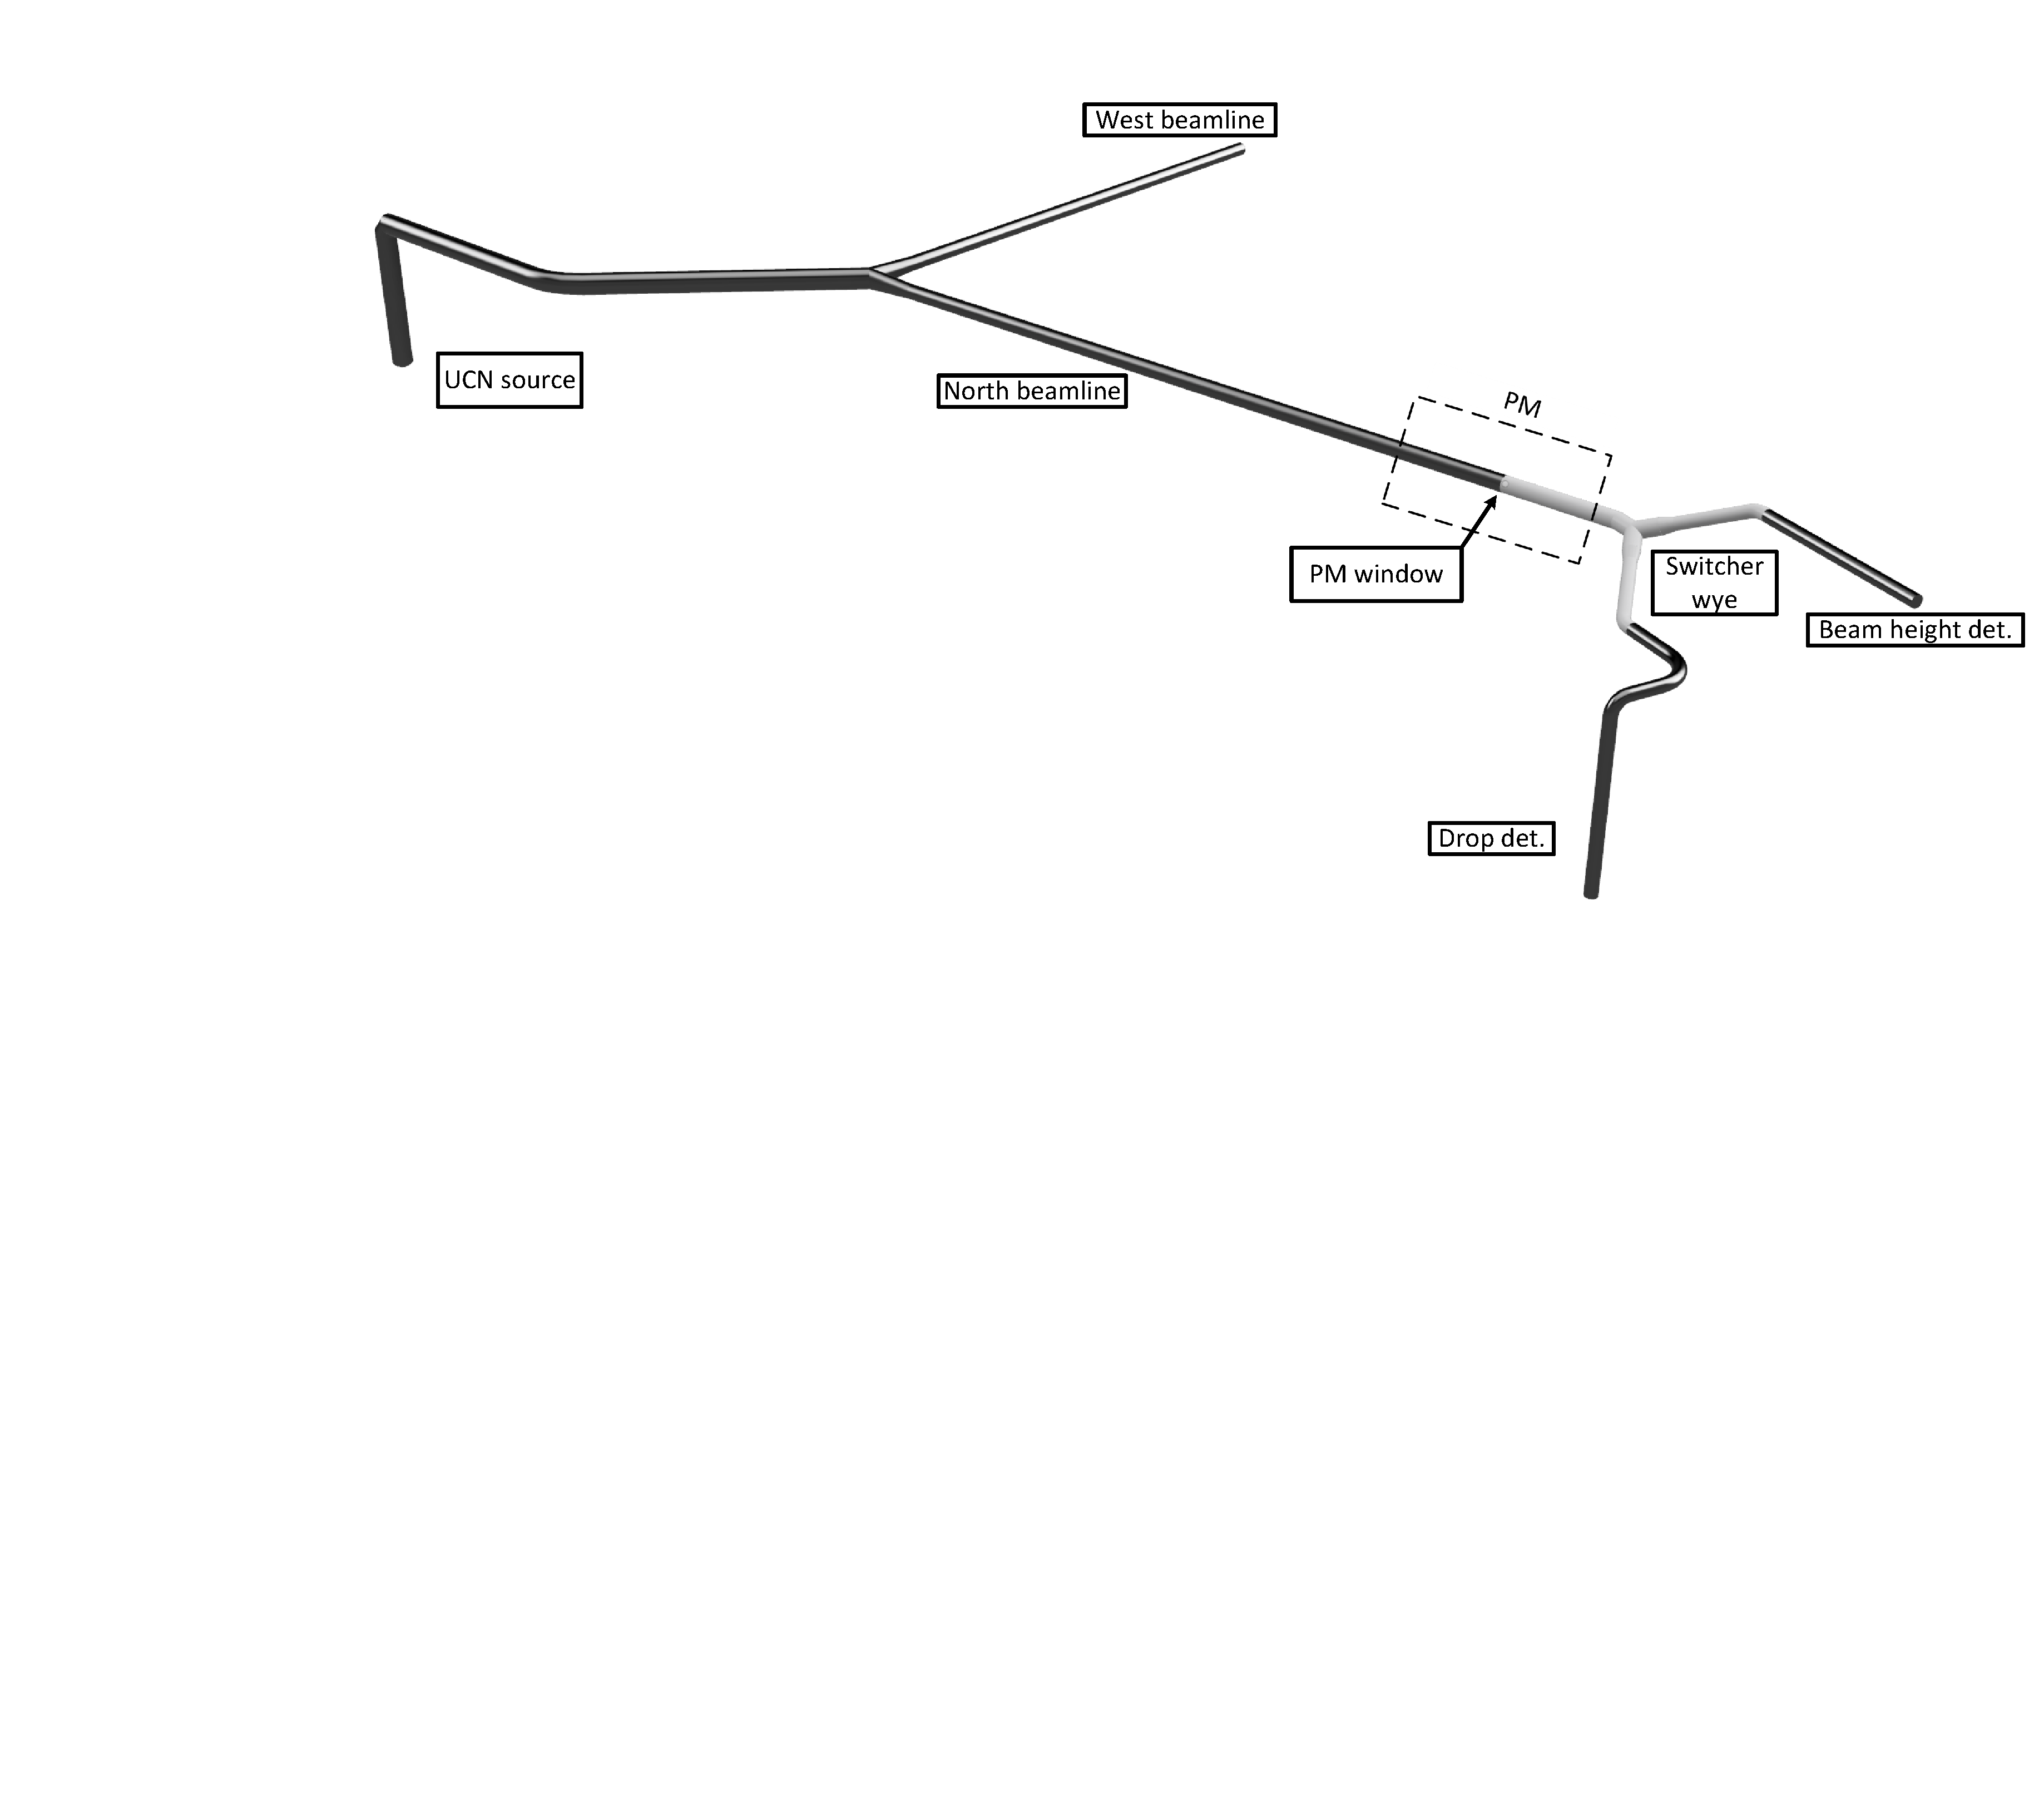
\includegraphics[width=\textwidth]{figures/2022_north_beamline_drop_pentrack.pdf}
    \caption
    {Experimental geometry of the LANL nEDM on the North beamline (Chap.~\ref{chap:nEDM_commissioning_dec2022}) used to test UCN spin transport in \pentrack. The lower switcher directs UCN from the wye into the drop detector}
    \label{fig:2022_beamline_pentrack_drop}
% \end{figure}
    \vspace{\baselineskip}
% \begin{figure}
    \centering
    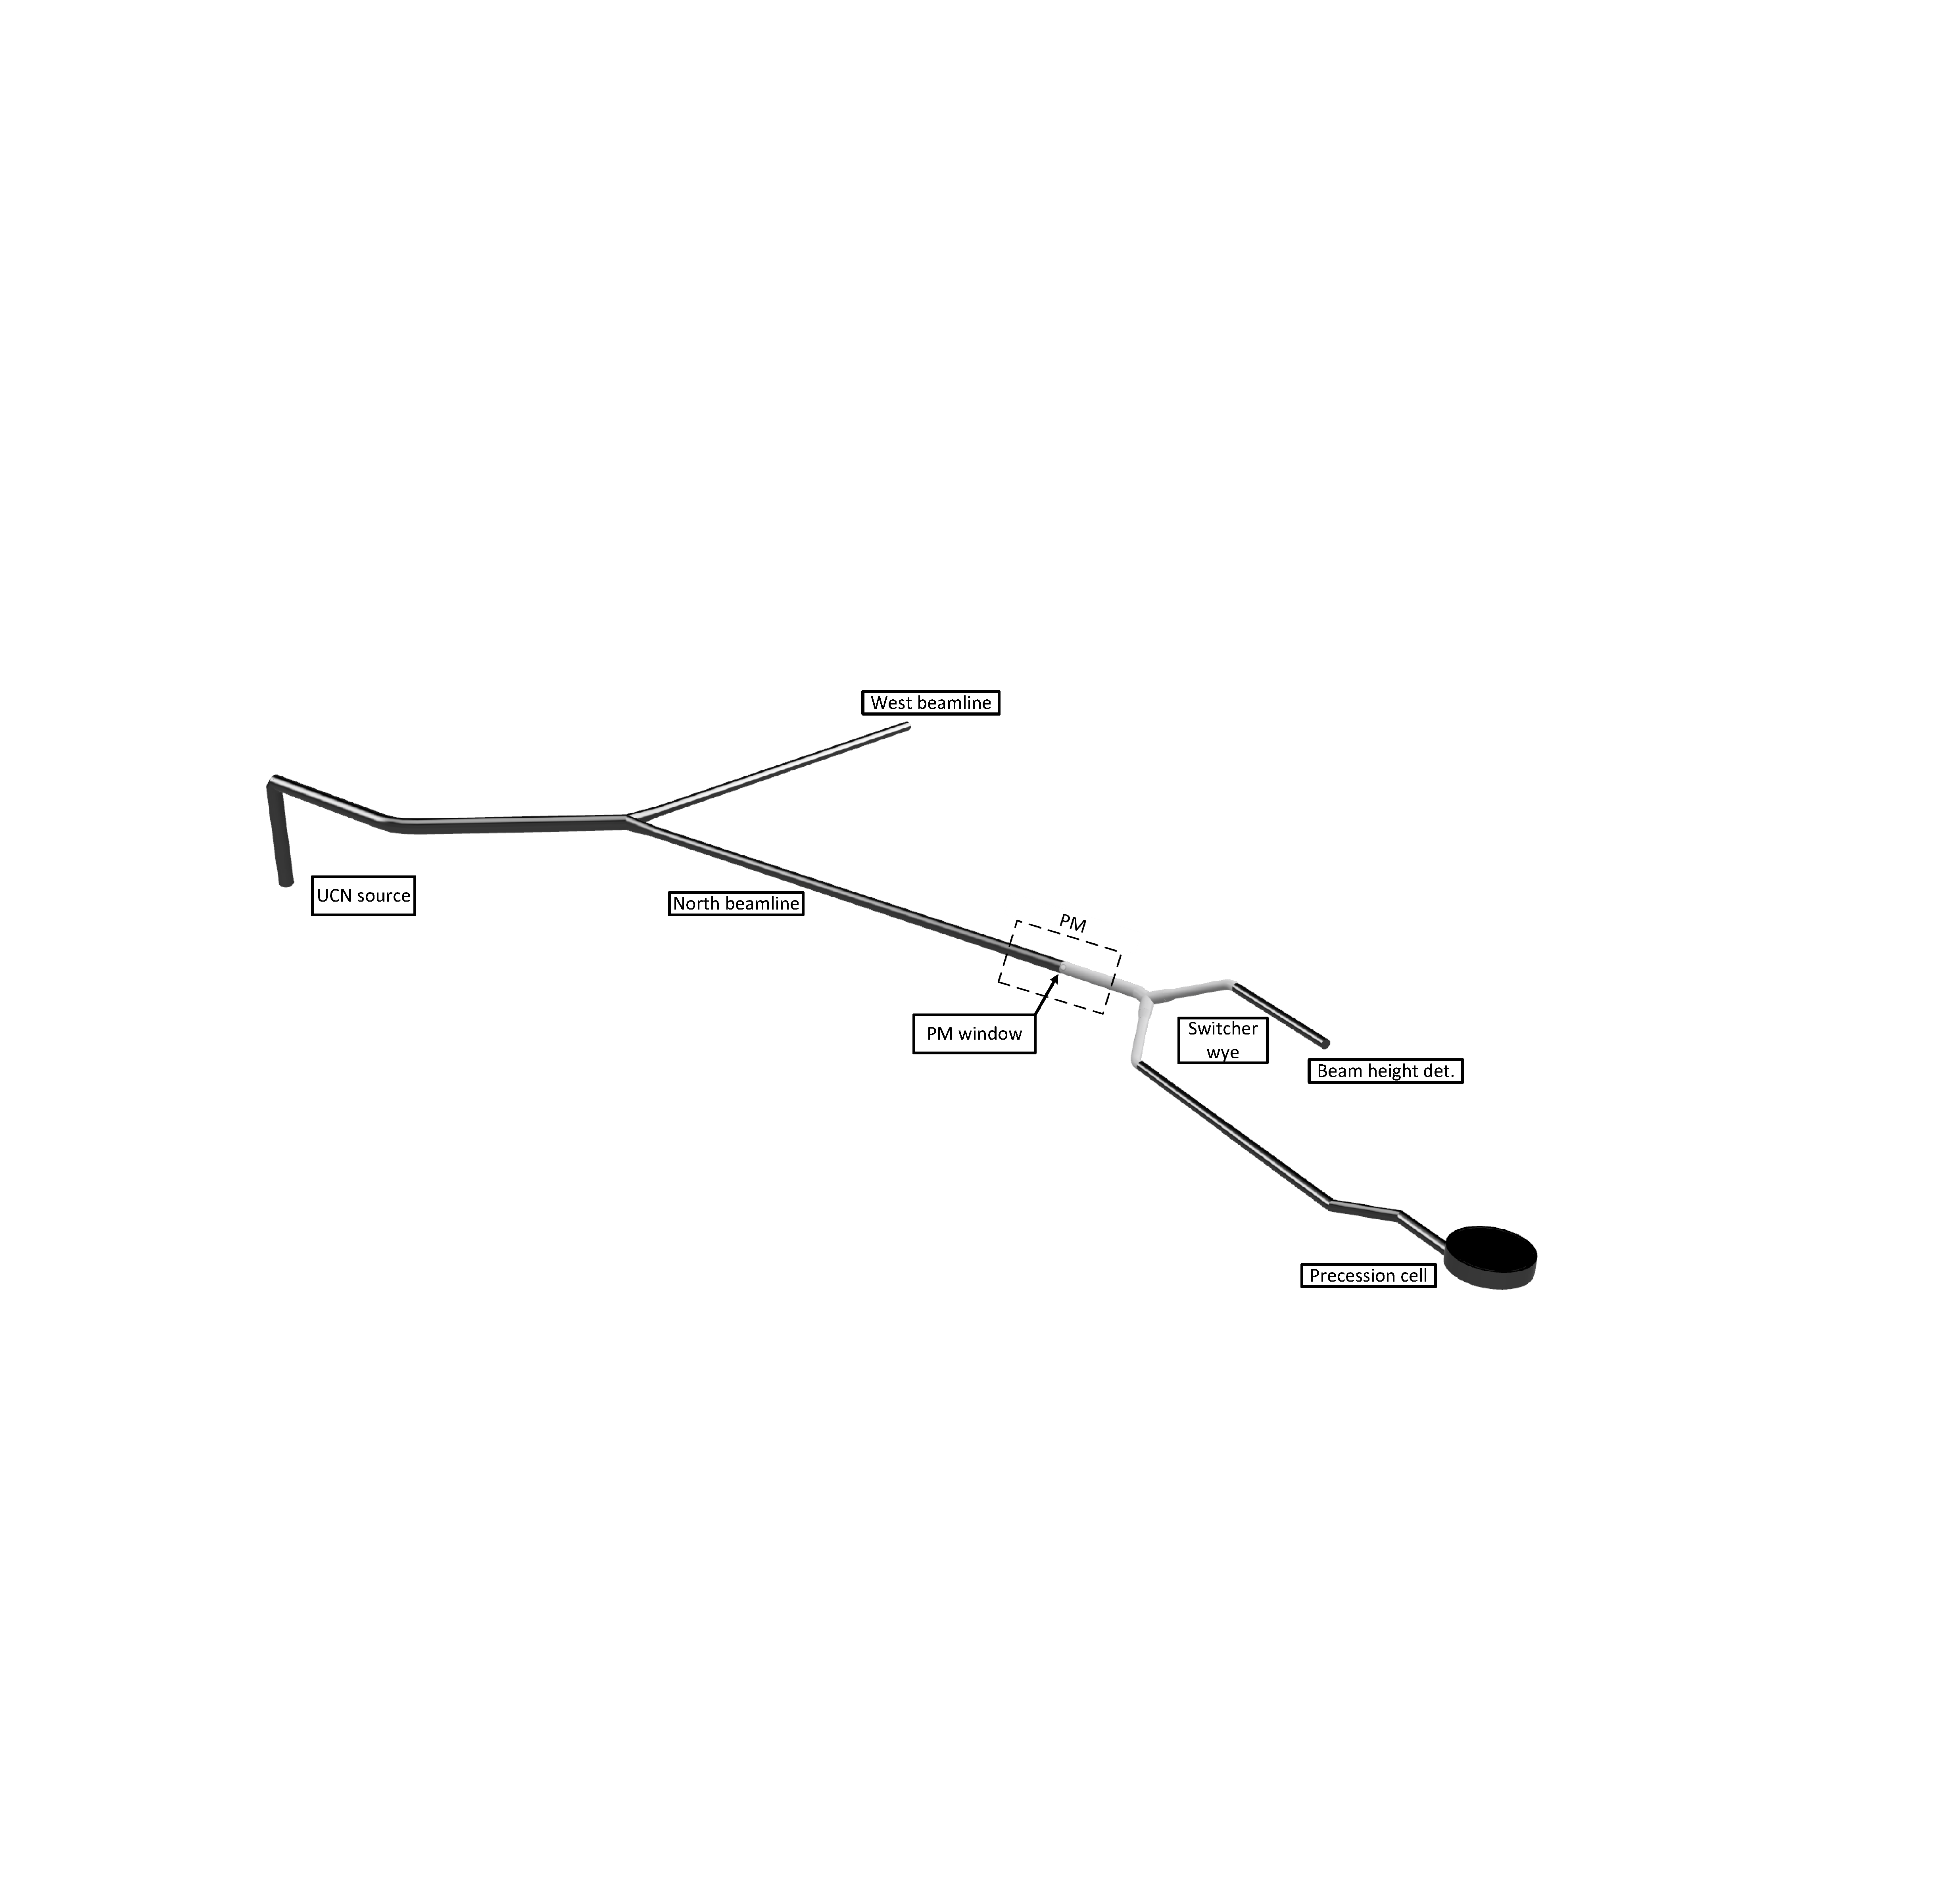
\includegraphics[width=\textwidth]{figures/2022_north_beamline_cell_pentrack.pdf}
    \caption{Experimental geometry of the LANL nEDM on the North beamline (Chap.~\ref{chap:nEDM_commissioning_dec2022}) used to test UCN spin transport in \pentrack. The lower switcher is in the filling mode}\label{fig:2022_beamline_pentrack_cell}
\end{figure}

\begin{figure}
\centering
%subfigure width gets "multiplied" by includegraphics width
\begin{subfigure}{.5\textwidth} 
  \centering
  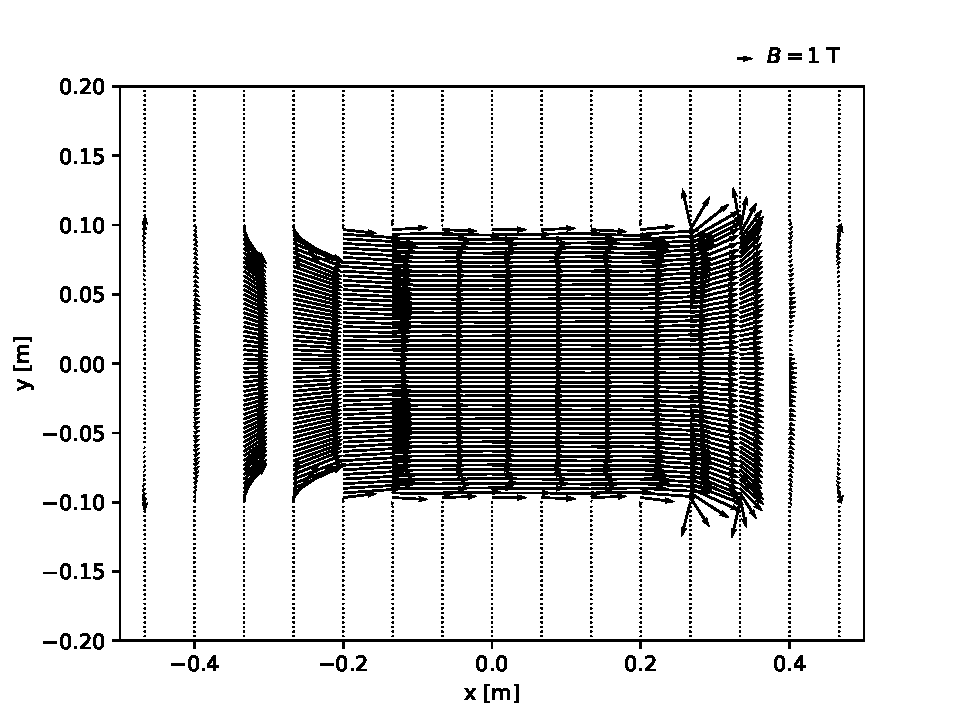
\includegraphics[width=\textwidth]{figures/PM_vector_field.pdf}
  \caption{}\label{subfig:PM_vector_field}
\end{subfigure}%DO NOT REMOVE THIS '%'
\begin{subfigure}{.5\textwidth}
  \centering
  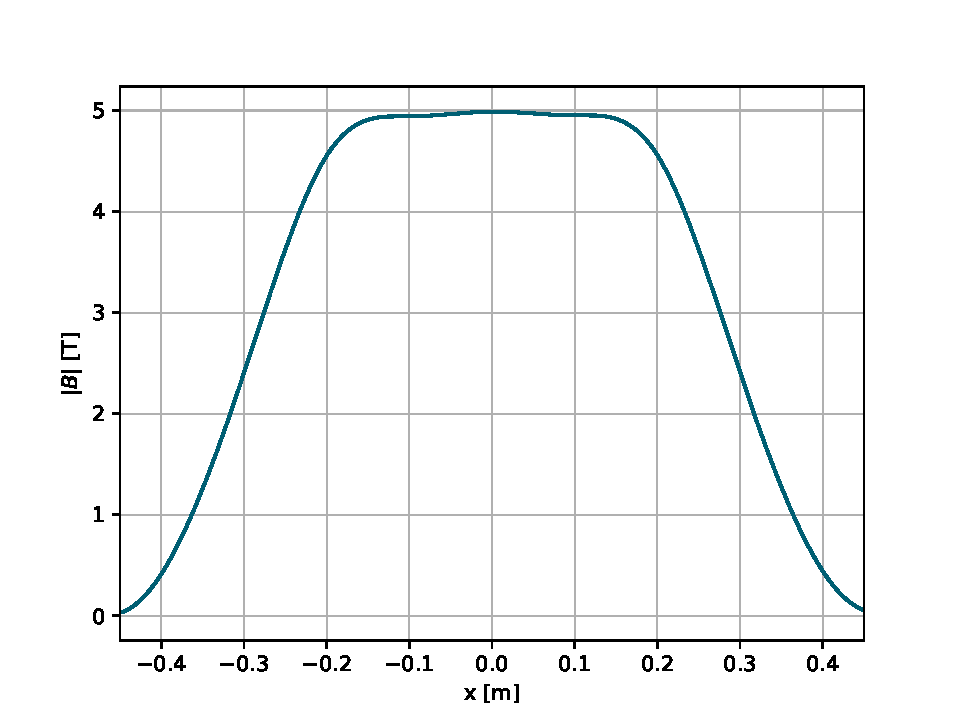
\includegraphics[width=\textwidth]{figures/PM_magnitude.pdf}
  \caption{}\label{subfig:PM_magnitude}
\end{subfigure}
\caption
[\textbf{(\subref{subfig:PM_vector_field})} Slice of the PM $\glsvv{B}$ field in Sec.~\ref{sec:switcher_wye_transport_monte_carlo}. Simulated data provided by the vendor. \textbf{(\subref{subfig:PM_magnitude})} Magnitude of the PM field along the center of the UCN beamline]
{\textbf{(\subref{subfig:PM_vector_field})} Slice of the PM $\vv{B}$ field used in Sec.~\ref{sec:switcher_wye_transport_monte_carlo}. Simulated data provided by the vendor. \textbf{(\subref{subfig:PM_magnitude})} Magnitude of the PM field along the center of the UCN beamline (oriented along $\vv{x}$)}
\label{fig:PM_field_simulated}
\end{figure}


\begin{figure}
\centering
%subfigure width gets "multiplied" by includegraphics width
\begin{subfigure}{.5\textwidth}
  \centering
  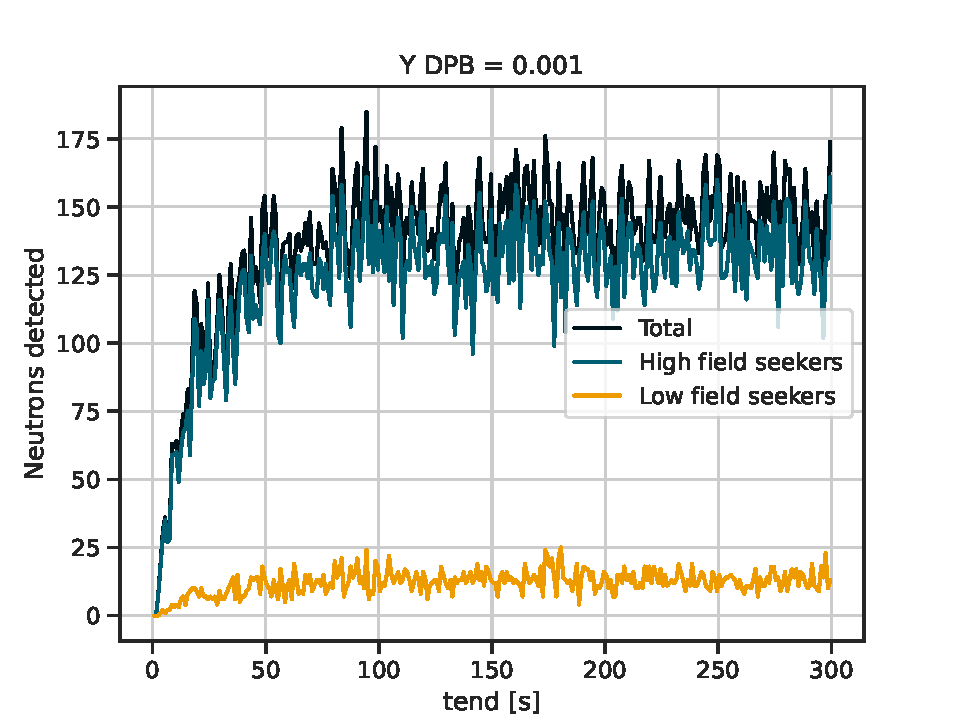
\includegraphics[width=\textwidth]{figures/flow_through_dpb_0.001.pdf}
  \caption{}\label{subfig:dpb_001}
\end{subfigure}%DO NOT REMOVE THIS '%'
\begin{subfigure}{.5\textwidth}
  \centering
  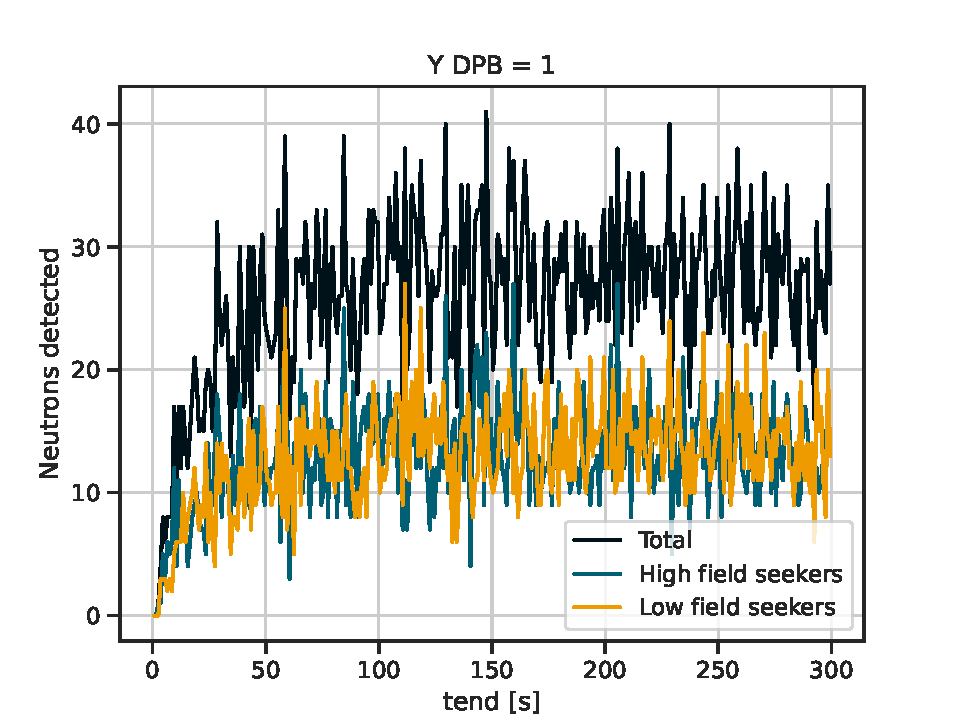
\includegraphics[width=\textwidth]{figures/flow_through_dpb_1.pdf}
  \caption{}\label{subfig:dpb_1}
\end{subfigure}
\begin{subfigure}{.5\textwidth}
  \centering
  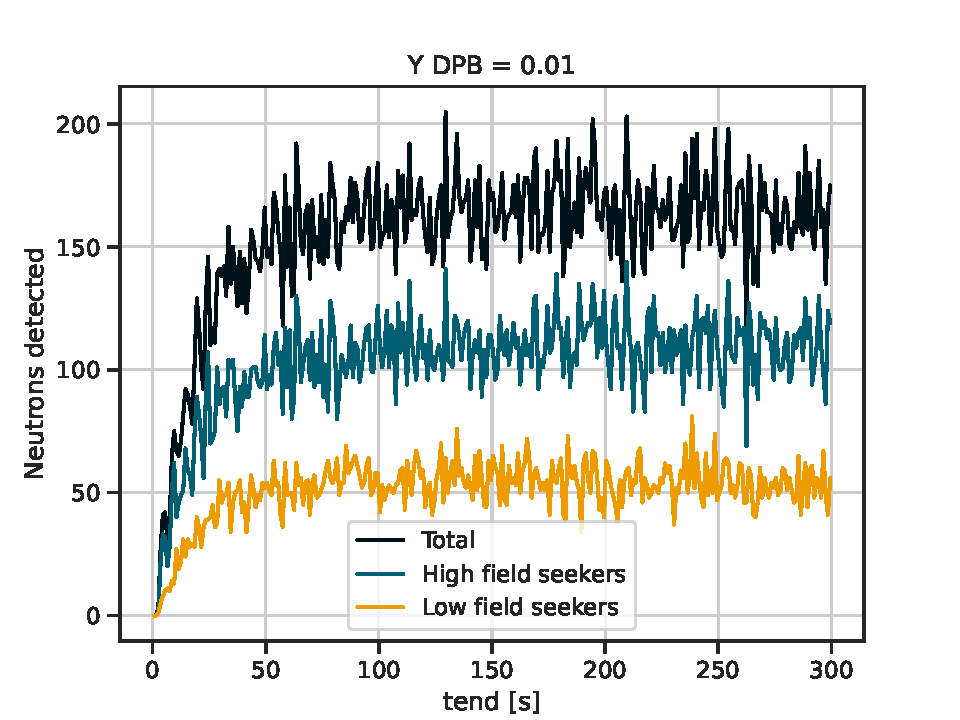
\includegraphics[width=\textwidth]{figures/flow_through_dpb_0.01.pdf}
  \caption{}\label{subfig:dpb_01}
\end{subfigure}
\caption
[Simulated UCN rate in the drop detector in a flow through mode, shown here for varying depolarization per bounce (DPB) in the switcher wye parameters.]
{Simulated UCN rate in the drop detector in a flow through mode, shown here for varying depolarization per bounce (DPB) in the switcher wye parameters. The $x$-axis value $t_\text{end}$ refers to the time at which the neutrons were detected. \textbf{(\subref{subfig:dpb_001})} $\text{DPB}=0.001$, UCN remain mostly polarized ($A\approx 1$). \textbf{(\subref{subfig:dpb_1})} $\text{DPB}=1$, UCN are completely depolarized ($A\approx 0$). \textbf{(\subref{subfig:dpb_01})} A 2:1 ratio of high field seekers to low field seekers gives ($A\approx 0.33$)}
\label{fig:dpb_flow_through}
\end{figure}



\begin{figure}
\centering
%subfigure width gets "multiplied" by includegraphics width
\begin{subfigure}{.5\textwidth} 
  \centering
  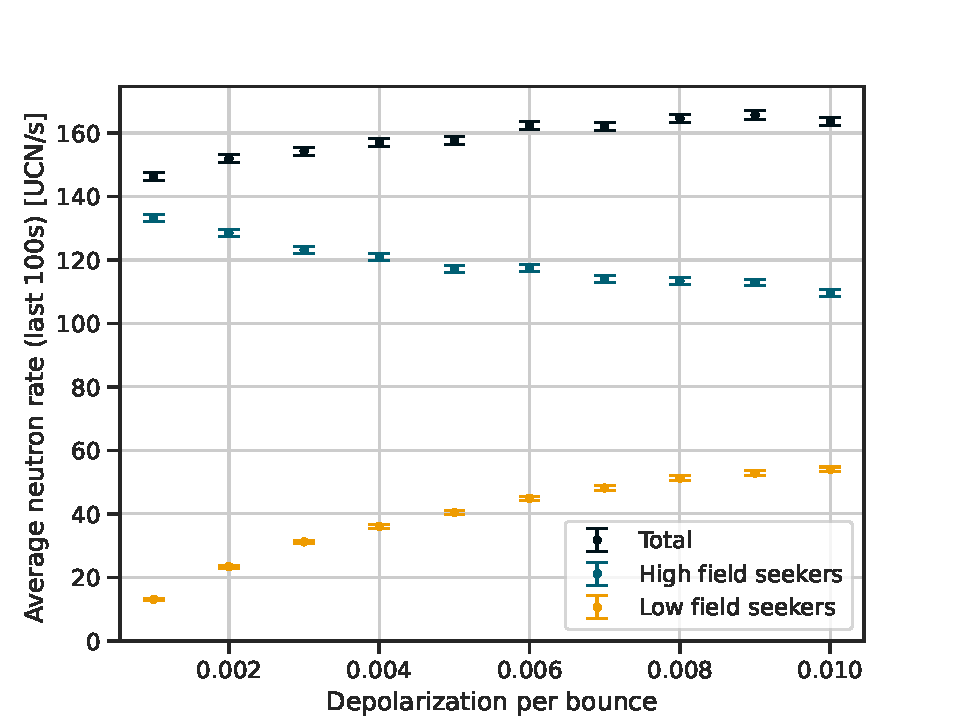
\includegraphics[width=\textwidth]{figures/flow_through_average.pdf}
  \vspace{0pt}
  \caption{}\label{subfig:pentrack_north_beamline_flow_through_average}
\end{subfigure}%DO NOT REMOVE THIS '%'
\begin{subfigure}{.5\textwidth}
  \centering
  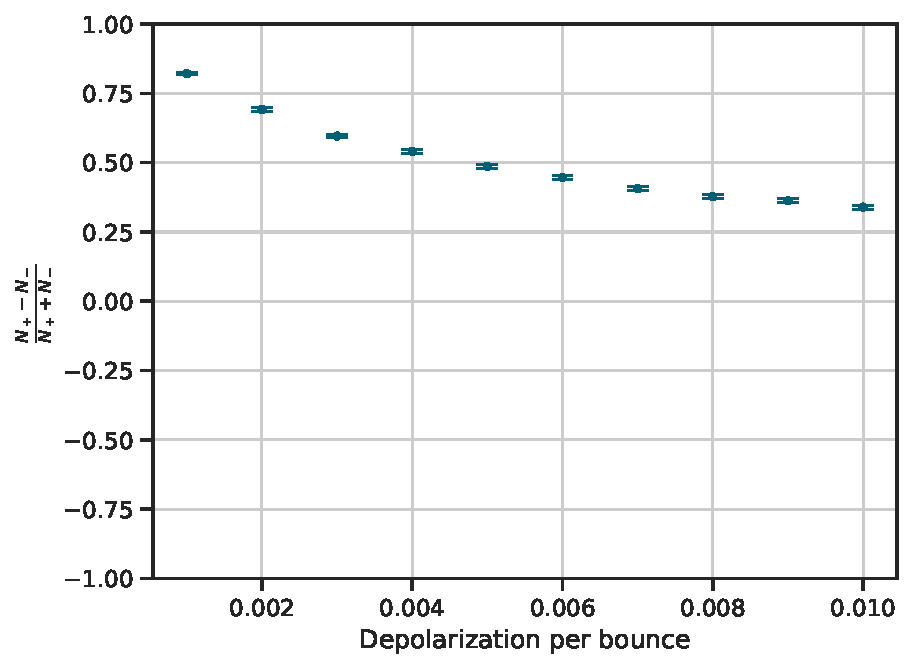
\includegraphics[width=\textwidth]{figures/flow_through_spin_contrast.pdf}
  \vspace{-7pt}
  \caption{}\label{subfig:pentrack_north_beamline_flow_through_asymmetry}
\end{subfigure}
\caption
    {\textbf{(\subref{subfig:pentrack_north_beamline_flow_through_average})} Simulated UCN rate in the drop detector as a function of depolarization per bounce in the switcher wye. \textbf{(\subref{subfig:pentrack_north_beamline_flow_through_asymmetry})} Asymmetry as a function of depolarization per bounce in the switcher wye.}
\label{fig:pentrack_north_beamline_flow_through}
\end{figure}

\begin{figure}
\centering
%subfigure width gets "multiplied" by includegraphics width
\begin{subfigure}{.5\textwidth} 
  \centering
  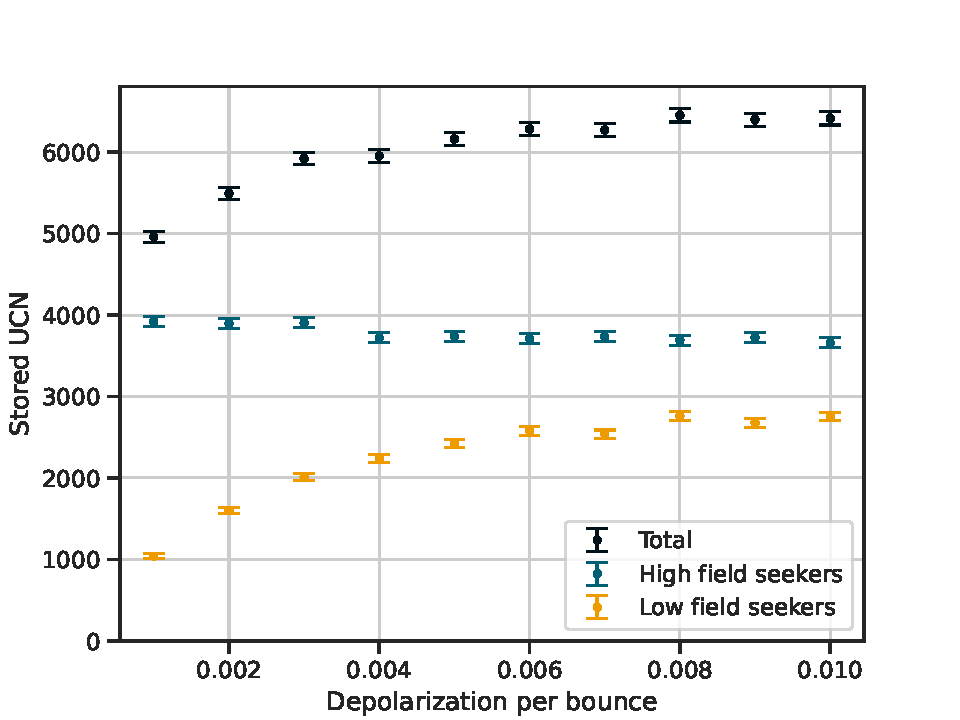
\includegraphics[width=\textwidth]{figures/stored_ucn.pdf}
  \vspace{0pt}
  \caption{}\label{subfig:pentrack_north_beamline_stored_counts}
\end{subfigure}%DO NOT REMOVE THIS '%'
\begin{subfigure}{.5\textwidth}
  \centering
  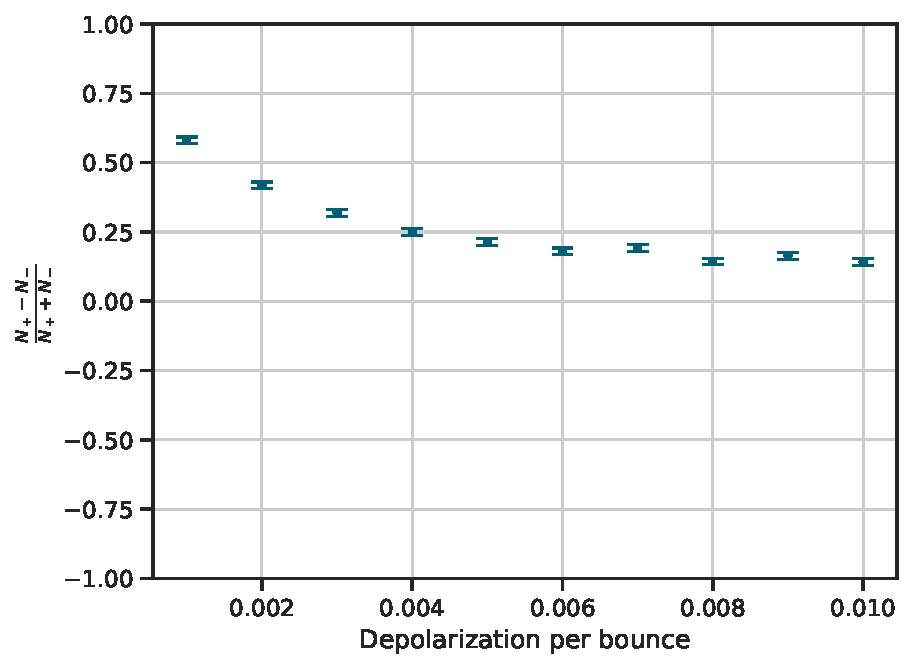
\includegraphics[width=\textwidth]{figures/storage_spin_contrast.pdf}
  \vspace{-7pt}
  \caption{}\label{subfig:pentrack_north_beamline_stored_asymmetry}
\end{subfigure}
\caption
    {\textbf{(\subref{subfig:pentrack_north_beamline_stored_counts})} Simulated counts of stored UCN in the precession cell as a function of depolarization per bounce in the switcher wye. \textbf{(\subref{subfig:pentrack_north_beamline_stored_asymmetry})} Asymmetry as a function of depolarization per bounce  in the switcher wye.}
\label{fig:pentrack_north_beamline_stored}
\end{figure}

\begin{figure}
\centering
%subfigure width gets "multiplied" by includegraphics width
\begin{subfigure}{.5\textwidth}
  \centering
  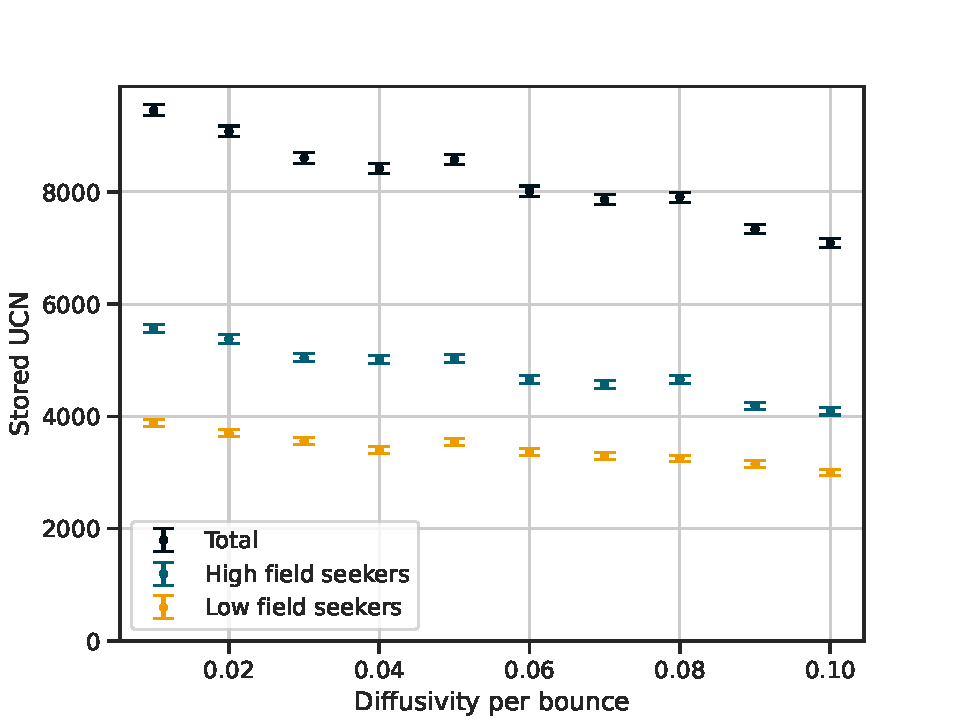
\includegraphics[width=\textwidth]{figures/stored_ucn_diffuse.pdf}
  \vspace{0pt}
  \caption{}\label{subfig:diffuse_storage_counts}
\end{subfigure}%DO NOT REMOVE THIS '%'
\begin{subfigure}{.5\textwidth}
  \centering
  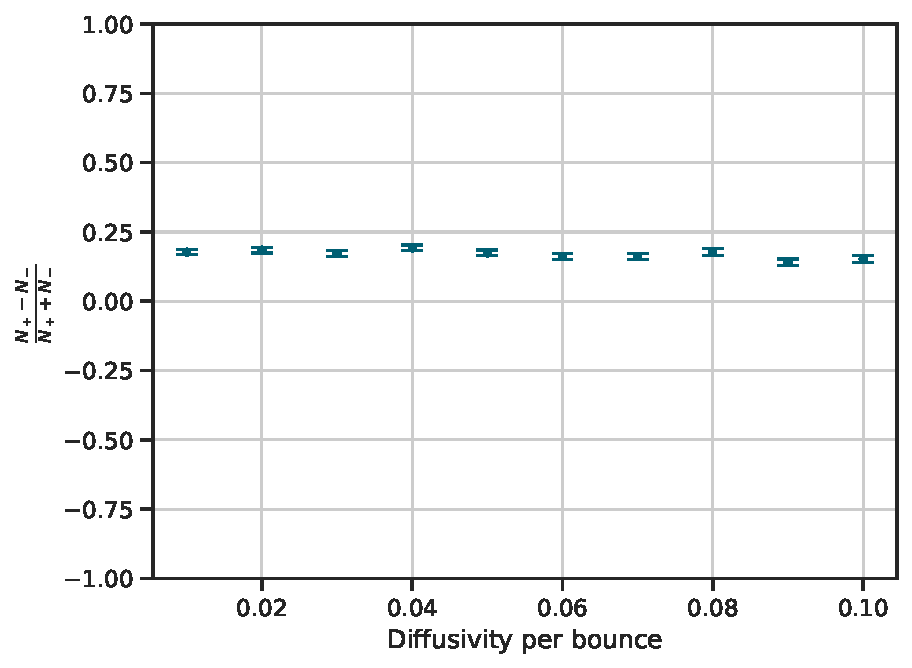
\includegraphics[width=\textwidth]{figures/storage_spin_contrast_diffuse.pdf}
  \vspace{-7pt}
  \caption{}\label{subfig:diffuse_storage_contrast}
\end{subfigure}
\begin{subfigure}{.5\textwidth}
  \centering
  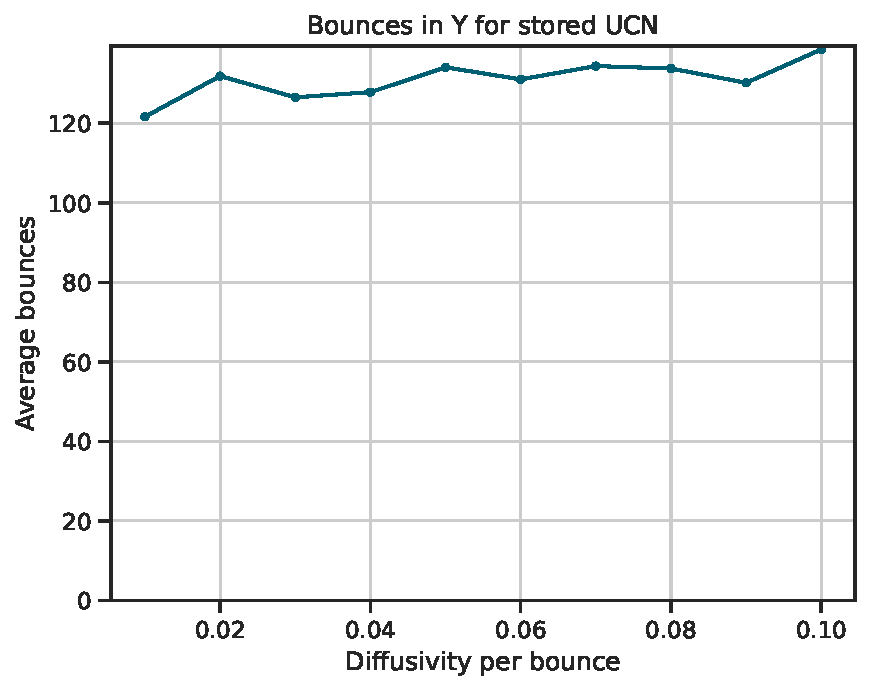
\includegraphics[width=\textwidth]{figures/average_bounces_in_y.pdf}
  \caption{}\label{subfig:average_bounces_in_y}
\end{subfigure}
\caption
[Simulated UCN storage in the precession cell as a function of (Lambertian) diffusivity probability in the switcher wye, with depolarization per bounce at $0.007$.]
{Simulated UCN storage in the precession cell as a function of (Lambertian) diffusivity probability in the switcher wye, with depolarization per bounce at $0.007$. Figs.~\textbf{(\subref{subfig:diffuse_storage_counts})} -- \textbf{(\subref{subfig:diffuse_storage_contrast})} plot stored UCN and calculated asymmetry as a function of diffusivity probability per bounce. Fig.~\textbf{(\subref{subfig:average_bounces_in_y})} describes the average number bounces in the switcher wye experienced by UCN that are in the cell by the end of the storage period}
\label{fig:diffusivity_study}
\end{figure}

We now turn to \pentrack simulations of the nEDM apparatus on the North beamline. In this section, we consider the possibility that depolarization in the switcher wye region limits spin asymmetry of stored UCN. We examine whether depolarization in the switcher wye region, which gave an asymmetry of $A\approx0.55$ for a flow through measurement to the drop detector (Fig.~\ref{fig:2022_single_arm_asymmetry}), could help explain the $A=0$ value measured for stored UCN (Tab.~\ref{tb:t1_2022_measurements}). If UCN encountered the depolarizing wye region enough times during the filling period it is possible that there would have a large impact on stored UCN spin asymmetry.

To reduce the need to adjust input UCN energy spectrum and related parameters, we generated UCN isotropically in the SD$_2$ source (Sec.~\ref{sec:lanl_ucn_source}) and simulated the entire beamline. The energy spectrum of generated UCN in the source was $v^3\,dv\,(=E\,dE)$, for UCN energies 0--\qty{250}{n\eV}, which reasonably emulated the spectrum reported in Ref.~\cite{saunders_performance_2013}. The source was run in a pulsed mode to mimic the delivery of the proton beam, generating UCN for \qty{0.7}{s} at \qty{5}{s} intervals. In addition, a thin material butterfly valve appeared above the source when the beam was ``not delivered'' to limit UCN reabsorption in the SD$_2$ (at the time of writing this dissertation, \pentrack does yet not support moving geometries, so the opening and closing process of the butterfly valve was instantaneous).

UCN leaving the source were directed up a \qty{1}{m} $\ce{^{58}Ni}$ guide, where NiP-coated guides directed UCN to either a blanked-off West beamline (SS gate valve) or the North beamline. UCN that reached the North beamline were subjected to a numerical PM (Sec.~\ref{sec:PM_description}) magnetic field, provided by the vendor and imported into \pentrack (Fig.~\ref{fig:PM_field_simulated}). An analytical \qty{50}{\micro T} ``transport field'' oriented along the North beamline was also applied globally within the simulation.

First, we simulated a flow-through measurement (Fig.~\ref{fig:2022_beamline_pentrack_drop}) where UCN on the lower detector were directed towards the drop detector where the drop detector had perfect detection efficiency. A depolarization per bounce (DPB) factor was applied to the switcher wye and treated as a free parameter, with the goal of matching the asymmetry measured from Sec.~\ref{sec:2022_single_arm_benchmarks}. As validation, Fig.~\ref{fig:dpb_flow_through} plots high-field seekers and low-field seekers counted by the drop detector as a function of time. In the limit that $\text{DPB}=1$, UCN were completely depolarized (equal rates of high-field seekers and low field seekers), and as DPB decreases there remain predominantly high-field seekers. Parameter sweeps (Fig.~\ref{subfig:pentrack_north_beamline_flow_through_asymmetry}) indicated that $\text{DPB}\approx \num{5e-3}$ could account for the observed asymmetry, which is quite high. As context, the loss per bounce parameter for NiP is on the order of $\sim 10^{-4}$~\cite{pattie_jr_evaluation_2017}. It is possible that the depolarization per bounce may be representing a magnetic field zero in the switcher wye region instead of a material source of depolarization.

We then proceeded to simulate a storage measurement, where the lower switcher was now directed to fill the precession cell (Fig.~\ref{fig:2022_beamline_pentrack_cell}). As with the measurements from Sec.~\ref{sec:2022_ucn_storage_measurements}), we used a fill time of \qty{50}{s} and a storage period of \qty{30}{s}. Guides between the switcher and the cell were designated as Cu, the cell wall was dPS, and the HV electrodes were NiP. UCN remaining in the precession cell at the end of the storage period were immediately counted with perfect efficiency. Fig.~\ref{subfig:pentrack_north_beamline_stored_asymmetry} shows the asymmetry of stored UCN as a function of the DPB. Asymmetry does appear to reach a fairly low value of $A\approx 0.1$ for $\text{DPB}\geq \num{6e-3}$, thus suggesting that depolarization in the wye could indeed be large contributing factor to the experimentally measured value of $A=0$ for stored UCN.

Proceeding with a nominal DPB value of \num{7e-3}, (Lambertian) diffusivity of the switcher wye (nominally $0.05$~\cite{pattie_jr_evaluation_2017}) was varied to determine whether UCN could spend longer periods of time in the depolarizing region. Results of UCN storage simulation are presented in Fig.~\ref{fig:diffusivity_study}. From Fig.~\ref{subfig:diffuse_storage_counts} we see that increasing diffusivity reduces the number of UCN that arrive at the cell. However, Fig.~\ref{subfig:diffuse_storage_contrast} indicates that the asymmetry is relatively insensitive to diffusivity. Fig.~\ref{subfig:average_bounces_in_y} plots the average number of bounces in the switcher wye for UCN that are in the chamber at the end of the filling period. Higher statistics would improve the the resolution of the trend line, but it appears that even the most generous interpretation gives an increase of 20 bounces in the wye per diffusivity probability increase of 10\%. Given a depolarization per bounce on the order of $\sim 10^{-3}$ this would not be enough to significantly affect asymmetry.

%%%%%%%%%%%%%%%%%%%%%%%%%%%%%%%%%%%%%%%%%%

\section{1D random walk}\label{sec:1D_random_walk}

%%%%%%%%%%%%%%%%%%%%%%%%%%%%%%%%%%%%%%%%%%

\begin{table}
\centering
\caption
{Example results from the 1D random walk model (Sec.~\ref{sec:1D_random_walk}). Each simulation uses \qty{1e6}{UCN}. Note that the number of window passes for UCN that make it to the cell must be an odd number}\label{tb:1D_random_walk}
\begin{tabular}{
    S[table-format = 1.2]
    S[table-format = 5.0]
    S[table-format = 6.0]
    S[table-format = 2.2]
}
\toprule
{\makecell{Single pass \\ loss per bounce}} & {UCN in cell} & {UCN lost on window} & {\makecell{Average window passes\\(for UCN in cell)}} \\
\midrule
0       & 86905 & 0 & 11.33 \\
0.01    & 77797 & 49732 & 10.42 \\
0.02    & 70453 & 91125 & 9.59 \\
0.03    & 63860 & 125476 & 8.90 \\
0.04    & 58698 & 156116 & 8.26 \\
0.05    & 53983 & 182420 & 7.74 \\
\bottomrule
\end{tabular}
\end{table}

The presence of the Al window in the PM region (Sec.~\ref{sec:PM_description}) results in the loss of some high field seekers from the Al total cross section, absorption from thin oxide films~\cite{pokotilovski_effect_2016}, and bulk elastic scattering from structural inhomogenieties. The effect is compounded when nonspecular bounces cause high field seekers to pass through the Al window region multiple times. We use a simple 1D random walk model to estimate the loss factor from an absorption or effective cross section. The C++ code used to produce the estimate in this section is available at [\url{https://github.com/dougUCN/randomWalk}].

The probability for a neutron to be absorbed in the bulk of the Al window in a single pass can be described using the Beer Lambert Law, Eq.~(\ref{eq:beer_lambert_law})
%
\begin{gather*}
   P_\text{abs}(v) = 1 - \exp \left( - \frac{\ell_\text{window} }{ \lambda_\text{mfp} } \right)
\end{gather*}
%
where $\ell_\text{window}$ is the thickness of the window (\qty{1e-4}{m}), and $\lambda_\text{mfp} = 1 / (N\,\sigma_\text{abs}(v))$ is the mean free path of absorption. $N$ is number density and $\sigma_\text{abs}(v)$ is the velocity-dependent neutron absorption cross section of the material. 

High-field seeking UCN gain approximately 300 neV from the PM field. Assuming UCN in the NiP guide have energies in the \qty{0}{n\eV} to \qty{214}{n\eV} range, high field seekers that encounter the PM window will be in the \qty{300}{n\eV} to \qty{513}{n\eV} regime. $P_\text{abs}(v)$ in this regime can be approximated with a flat line, and we estimate $P_\text{abs}\approx 0.03$ for a single pass through the window.

The UCN path from the source to the cell can be modeled as a 1D random walk, where the step size is the distance traveled by a particle before a nonspecular bounce. From Eqs.~(4.79), (4.70), and (4.48) in Ref.~\cite{golubUCN}, we write
%
\begin{gather}
    d = 2 R\sqrt{\frac{2(2-P_\text{nonspec})}{3P_\text{nonspec}} }
\end{gather}
%
where $R=\qty{1.5}{in}=\qty{0.0381}{m}$ is the radius of the cylindrical UCN guide and $P_\text{nonspec}$ is the probability of a Lambertian (Sec.~\ref{sec:diffuse_reflections}) bounce. Nonspecularity for NiP-coated \acrshort{ss} pipes has previously been measured to be $P_\text{nonspec}\approx0.05$~\cite{pattie_jr_evaluation_2017}, but for Cu or NiP-coated Al, nonspecularity may be treated as a free parameter. For this example calculation we let $P_\text{nonspec}\approx0.05$, giving $d\approx \qty{0.389}{m}$.

NiP has a loss per bounce of $\sim 10^{-4}$~\cite{pattie_jr_evaluation_2017}. The loss per 1D step is then given by
%
\begin{align}
    \text{loss per step} &= 1 - \left(1 - \text{loss per bounce} \right)^{N_\text{spec}}\\
    &\approx N_\text{spec} \times \text{loss per bounce}
\end{align}

When a neutron reaches the end of the 1D beamline, the probability of it entering the cell is dictated by the ratio of the size of the cell entrance to the ``surface area'' of the last 1D step. We model this as
%
\begin{align}
    \text{cell entry chance} &= \left(1 - \left( 1 - \frac{ \text{area of the cell entrance} } {\text{surface area of last 1D step}} \right) ^ {N_\text{spec}} \right)^2 \\
    &= \left(1 - \left( 1 - \frac{ R_\text{entrance}^{2} } {2 R \, d} \right) ^ {N_\text{spec}} \right) ^2\label{eq:cell_entry_chance}
\end{align}
%
where the average number of specular bounces between a nonspecular bounce is given by $N_\text{spec} = 1/P_\text{nonspec}$. For a cell entrance radius $R_\text{entrance}=\qty{1.47}{in}=\qty{0.0373}{m}$ and $N_\text{spec}=20$ we estimate that the chance of entering the cell  is $\approx 0.38$.

Neutrons that enter the cell have a probability of exiting the cell before the end of the filling period. Assuming cell trajectories are isotropic in the cell, this ``exit lifetime'' can be approximated by
%
\begin{gather}
    \text{cell exit lifetime} = \frac{4V_\text{cell}}{\pi R_\text{entrance}^2 \bar{v}}
\end{gather}
%
derived using Eq.~(\ref{eq:effusion-lifetime}). $V_\text{cell}$ is the volume of the precession cell and $\bar{v}$ is the average of velocity of UCN in the cell. For a $v^2\,dv$ distribution (Sec.~\ref{subsec:storageCurves}) and NiP-coated guides (which store UCN up to $\qty{214}{neV}\approx\qty{6.4}{m\per s}$), 
%
\begin{gather}
    \bar{v}=\frac{\int_0^{6.4}{v^3\,dv}}{\int_0^{6.4}{v^2\,dv}}\approx \qty{4.8}{m\per s}
\end{gather}
%
In this example we let the UCN source be located at \qty{0}{m}, and the Al window at \qty{9}{m}, and the cell entrance at \qty{12}{m}. Assuming a preload procedure (Sec.~\ref{subsec:holdingTimeMeasurement}) was followed we let UCN start at the location of a gate valve on the beamline, located at \qty{6}{m}. For a fill time of \qty{50}{s}, UCN with a velocity $\bar{v}$ undergo the 1D random walk until the filling period is over. UCN that return to the D$_2$ source are considered to be lost. UCN that make it to the cell valve location may enter the cell based on Eq.~(\ref{eq:cell_entry_chance}). Neutrons that enter the cell remain for the duration of the cell exit lifetime and exit unless the fill time is completed.

Table~\ref{tb:1D_random_walk} illustrates some example results from the random walk for different single-pass window loss probabilities. To obtain more meaningful results, further studies are required, including the varying of diffusivity, beamline configuration, neutron velocity, and other parameters. 

The improvement of the model also requires comparison with experimental data. Due to the lengthy window removal and installation procedures, measurements on the North beamline in its current configuration without the window have been postponed. With regards to the data in Chap.~\ref{chap:north_beamline_paper}, the alterations in the preload procedure and guide configuration between run conditions was minor enough to allow for the comparisons presented in Sec.~\ref{sec:north_beamline_discussion}, but noticeable enough to obscure the window loss factor.

